\documentclass[12pt]{report}

%% Language and font encodings
\usepackage[english]{babel}
\usepackage[utf8x]{inputenc}
\usepackage[T1]{fontenc}

%% Sets page size and margins
\usepackage[top=3cm,bottom=2cm,left=3cm,right=3cm,marginparwidth=1.75cm]{geometry}

%% times new roman
\usepackage{newtxtext,newtxmath}

%% Useful packages
\usepackage{amsmath}
\usepackage{graphicx}
\usepackage[colorinlistoftodos]{todonotes}
\usepackage[colorlinks=true, allcolors=black]{hyperref}

% Specify bibliography package
\usepackage{natbib}

\usepackage{url}
\usepackage{mathptmx}


\title{Contemporary Issues in Developing Countries: \\Empirical Report}
\author{Naoto Nishida\\201811433\\ Media Arts, Science and Technology Department, University of Tsukuba}
\date{2021/12/21}



\begin{document}
% \renewcommand{\chaptername}{Day}
\maketitle
\tableofcontents

\chapter{Introduction}

So far, COVID-19 is overwhelming the whole over the world.
Researchers has been conducted surveys and analysis about COVID-19, such as the factors of Covid-19 infections or fatalities~\cite{toya2021cross,tsubasa2021modeling}, the effects of social distancing~\cite{CATO202051}, and relationships between COVID-19 positives and going-out-ratio accordingly to generations and genders.
However, there's been no research on relationships between COVID-19 and other diseases. 

UNAIDS, which is a NGO organization to promote global actions on HIV/AIDS pandemic, has posted an instructional report on how people with HIV should do to prevent themselves from COVID-19 infection~\cite{unaids, unaids_report}.
This organization studies mainly on practical knowledge that people should behave.

Therefore, in this report, I studied the relationship between COVID-19 and HIV, and other diseases in terms of the number of yearly incidence of positives. 


I assume that, if countries can keep the figures of positive cases of contagious diseases on a daily basis, they can immediately lower the number of COVID-19 positive cases in a year.
In addition, if people try to protect themselves from COVID-19 and keep social distancing or home staying, there should be a decrease in the number of other contagious diseases.
Thereby, my hypothesis is "there should be some relationships between the number of incidence of positives in each diseases and the transition of the number of COVID-19 cases in every country".

\chapter{Data}

In this chapter, I explain the datasets I used to study this hypothesis.
I used 
\begin{enumerate}
    \item Population, total(Population estimates and projections) in 2018 from DataBank~\cite{databank}
    \item Incidence of HIV, total (per 1,000 uninfected population) in 2020 from DataBank~\cite{databank}
    \item Incidence of malaria (per 1,000 population at risk) in 2020 from DataBank~\cite{databank}
    \item Incidence of tuberculosis (per 1,000 population at risk) in 2020 from DataBank~\cite{databank}
    \item Incidence of COVID-19 cases (Cumulative number) in 2020 and 2021 from Our World in Data~\cite{ourworldindata}
\end{enumerate}

In the 5th data above, I used a cumulative data of incidence of positives on 2021/12/24 and 2020/12/31 in order to get a sum of cases by year.
I organized data above by deleting row data of countries which don't exist on all datasets above.
% Then I put 0 to every missing data place, which is called single imputation. 
All of the data above is cross section data. 
The number of observations was 193.


The organized dataset and my project file are available at my GitHub repository\cite{github}

\chapter{Analytical Framework}

\begin{figure}
    \centering
    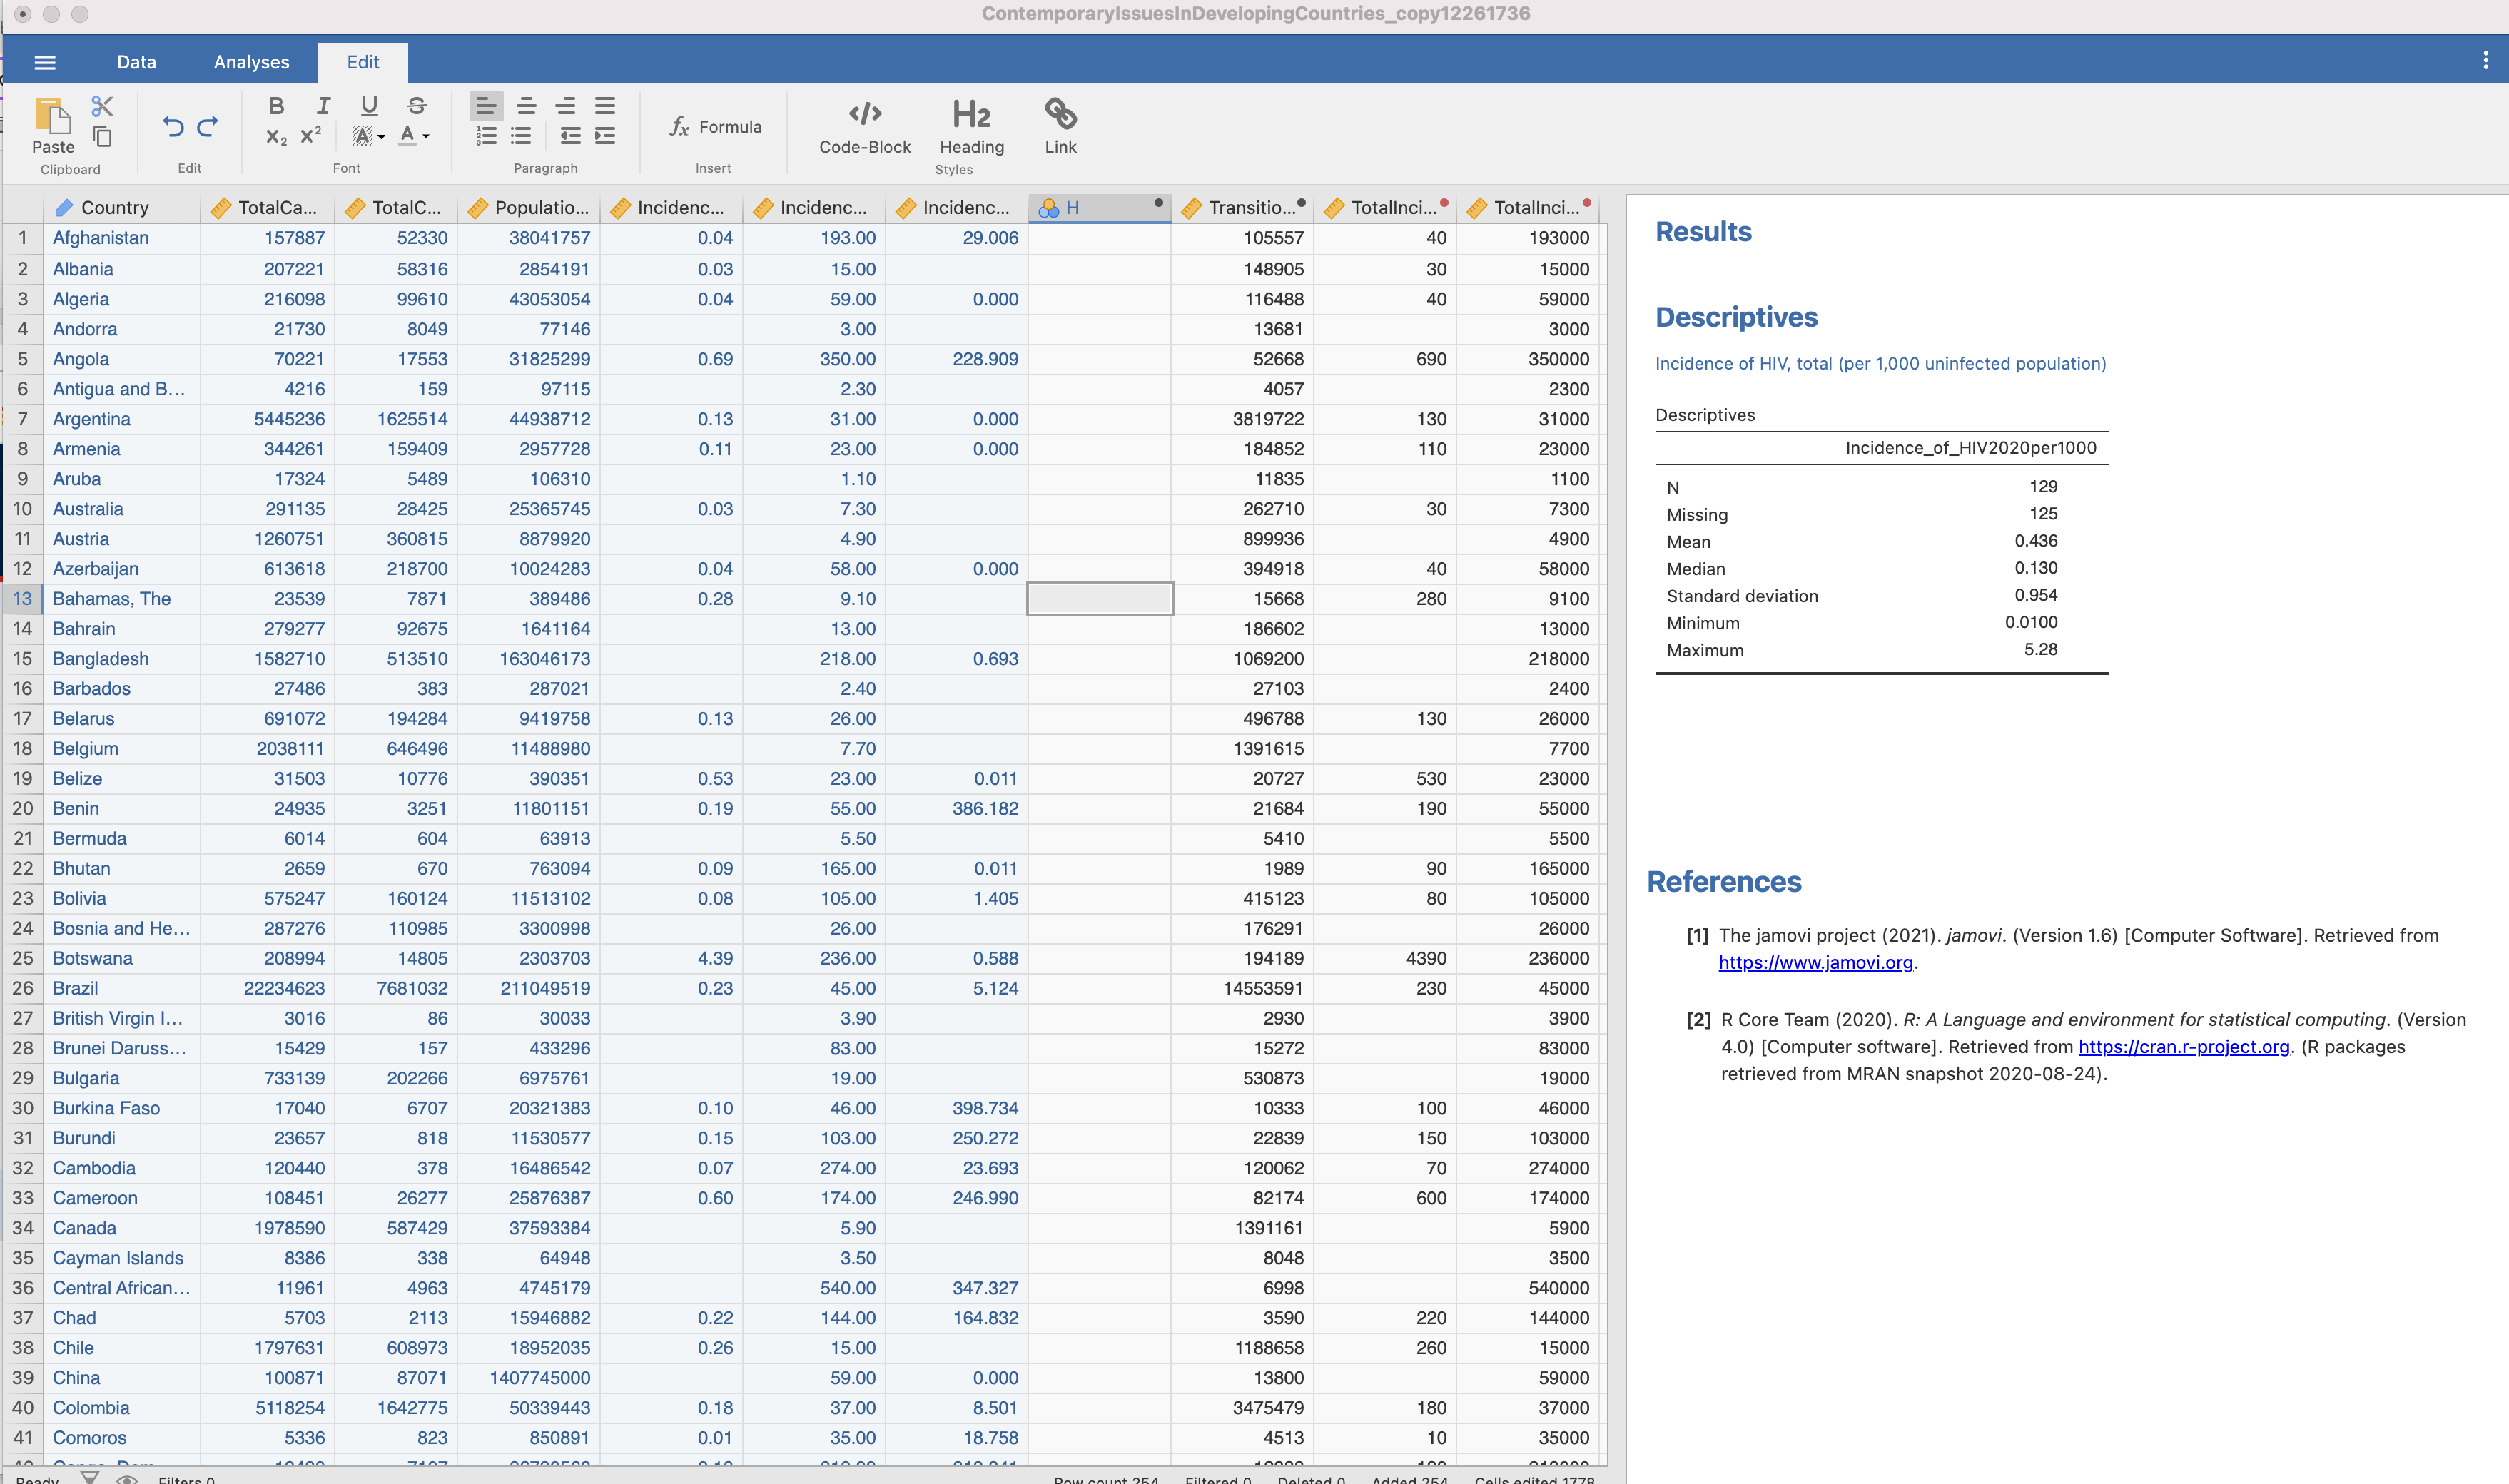
\includegraphics[width=140mm]{img/jamovi.png}
    \caption{Jamovi's user interface}
    \label{fig:jamovi}
\end{figure}

My hypothesis is "there should be some relationships between the number of incidence of positives in each diseases and the transition of the number of COVID-19 cases in every country".
I used a computed variable that suggests the number of cases, which calculated from the relative data (per 1,000 population).

My estimation model is below:

\begin{equation}
    T_c = I_{HIV}\beta_H + I_{Malaria}\beta_M + I_{TB}\beta_T + P\beta_P
\end{equation}

{\it{T}} means that the transition of the number of COVID-19 cases from 2020 to 2021.
{\it{c}} means each countries.
{\it{$I_{HIV}$}} means that the incidence of HIV cases.
{\it{$I_{Malaria}$}} means that the incidence of Malaria cases.
{\it{$I_{TB}$}} means that the incidence of tuberculosis cases.
{\it{$P$}} means the population of the country.
Each {$\beta$} is a coefficient.
{\it{T}} and {\it{P}} are integer, ratio scale variables.
{\it{c}} is a text, nominal variable.
The other four variables are decimal, ratio scale.

My estimation model is OLS.

In implementation, I used jamovi, which is a rapper software of R~\cite{jamovi} (figure~\ref{fig:jamovi}).



\chapter{Results and Discussion}
\begin{table}[h]
    \centering
    \begin{tabular}{lcc}
    \hline Model & $\mathrm{R}$ & $\mathrm{R}^{2}$ \\
    \hline 1 & $0.889$ & $0.791$ \\
    \hline
    \end{tabular}
    \caption{Model fit measures.}
    \label{tab:r}
\end{table}


\begin{table}[h]
    \centering
    \begin{tabular}{lrrrr}
    \hline \multicolumn{1}{c}{ Predictor } & Estimate & \multicolumn{1}{c}{ SE } & \multicolumn{1}{c}{$\mathrm{t}$} & $\mathrm{p}$ \\
    \hline Intercept & $437831.8479$ & $249245.93132$ & $1.757$ & $0.083$ \\
    Population2019 & $0.0181$ & $0.00104$ & $17.367$ & $<.001$ \\
    IncidenceOfMalaria2018per1000 & $-2203.2547$ & $1201.33898$ & $-1.834$ & $0.070$ \\
    IncidenceOfTB2020per1000 & $-1953.2374$ & $1307.77723$ & $-1.494$ & $0.139$ \\
    IncidenceOfHIV2020per1000 & $152995.3594$ & $173369.21225$ & $0.882$ & $0.380$ \\
    \hline
    \end{tabular}
    \caption{Model Coefficients}
    \label{tab:coefficient}
\end{table}

The result is above~\ref{tab:r}\ref{tab:coefficient}. 
There looks no significant effects on the transition of the number of COVID-19 cases from 2020 to 2021 from the coefficients related to diseases.
I assume that this result was because people may get such diseases in various way. For example, you may get COVID-19 easily even if you breath in the virus once, but you cannot get HIV virus in such way. In addition, I assume there were so many missing values in the dataset.
% Besides that, I cannot think of any other reasons, because I thought this model should work, actually.


\chapter{Conclusion}
The purpose of my study was to prove the hypothesis "there should be some relationships between the number of incidence of positives in each diseases and the transition of the number of COVID-19 cases in every country".
I supposed if countries can keep the figures of positive cases of contagious diseases on a daily basis, they can immediately lower the number of COVID-19 positive cases in a year.
The result was not that significant, but my suggestion should spot a light on the needs to survey of the relationships and co-effects of each diseases.





% For each day of class, you will have a new chapter
% \chapter{Thursday 19 January 2017: Introduction to Machine Translation}

% You should have one section per assigned reading
% \section{Is Translation an Art or a Math Problem?}

% Within each section, write a summary of that reading.
%
% Use \citet to cite a source inline
% Use \citep to cite a source parenthetically

% \todo{This is a todo note, pointing to an example of citing a source inline. Your final text should not include todo notes}
% \citet{lewiskrauss2015} makes the case that \ldots


% \section{Language: Finding a Voice}

% Sample sentence explaining something interesting \citep{greene2017}.

% \todo[inline]{This is an inline todo note, pointing to an example of citing a source parenthetically. Your final text should not include todo notes.}


% \section{A Neural Network for Machine Translation, at Production Scale}

% \todo[inline]{For each required reading, you should write a short review of the reading. The exact length will vary based on the length of the reading, but will typically be two or three paragraphs. Very short readings may have shorter reviews, and long readings may need to be a bit longer.}

% \section{Zero-Shot Translation with Google’s Multilingual Neural Machine Translation System}

% % \todo[inline]{Every section should cite the corresponding reading.}


\bibliographystyle{plain}
\bibliography{references}

\end{document}